\begin{center}

  \begin{tabular}{rp{16cm}lp{20cm}}%{rl}

  % after \\: \hline or \cline{col1-col2} \cline{col3-col4} ...

  论文地址:& \href{https://www.ijcai.org/Proceedings/2017/0239.pdf}{https://www.ijcai.org/Proceedings/2017/0239.pdf} \\
  来源:& IJCAI, 2017 \\
  作者:& Huifeng Guo, Ruiming Tang, et al. \\

  %源码:& \href{xxx}{xxx} \\

%  slides:& \href{http://yunshengb.com/wp-content/uploads/2017/03/nips_2018_r2l_workshop_talk.pdf}{{\footnotesize Convolutional Set Matching for Graph Similarity}}\\

  关键词:& \textbf{CTR, FMs, Wide\&Deep} \\

  写于:& \date{2021-08-31}

  \end{tabular}

\end{center}

该论文\cite{huifeng2017deepfm}提出了基于FM的深度模型 --- DeepFM,用于解决CTR问题。DeepFM与Wide\&Deep模型很像,但也有一些不同。DeepFM将Wide\&Deep中的LR替换为FM;不需要做特征工作;Wide和Deep部分的输入是共享的。

\paragraph{问题定义}
针对CTR问题,样本的特征可以分成多个field,$x = [x_{field_1}, x_{field_2}, ..., x_{field_m}]$,$x_{field_i}$是$field i$的向量表示,如one-hot编码。 

\paragraph{DeepFM}
DeepFM的整体结构如Fig.\ref{fig:deepfm}所示。DeepFM由两个部分组成:FM component和Deep component,这两部分共享输入。自底向上模型包含了Sparse Feature、Dense Embedding、FM Layer、Hidden Layer和Output Units。

对于Sparse Feature中的每一个特征,有一个权重与之相乘得到线性部分,也就是一阶特征;特征隐向量用于计算交叉特征之间的重要性,也就是二阶特征。特征隐向量也会作为Deep部分的输入。FM的输出与Deep的输出相加后经过Sigmoid函数后得到最终的输出。
$$
\hat{y} = sigmoid(y_{FM} + y_{DNN})
$$

\begin{figure}[h]
	\centering
	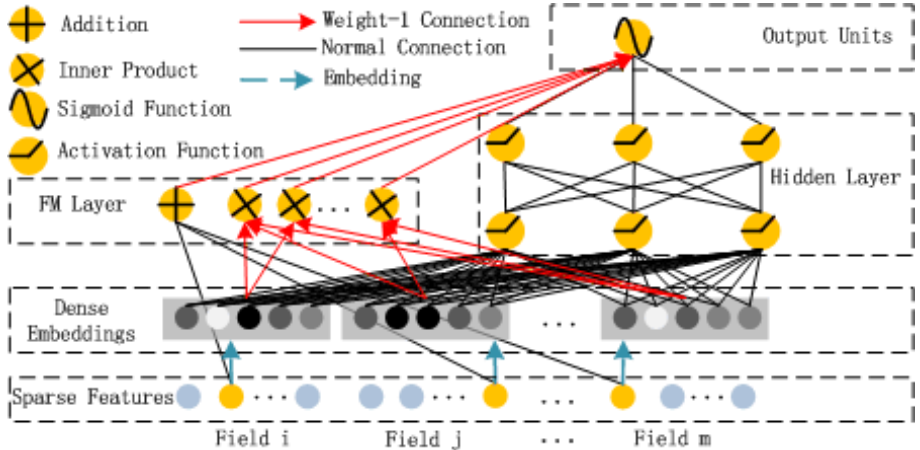
\includegraphics[width=.8\textwidth]{pics/deepfm.png}
	\caption{Wide \& deep architecture of DeepFM}
	\label{fig:deepfm}
\end{figure}

\subparagraph{FM Component}
\begin{figure}[h]
	\centering
	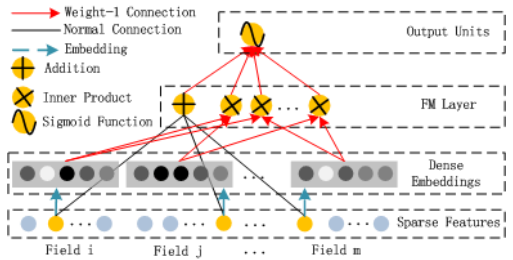
\includegraphics[width=.8\textwidth]{pics/deepfm-fm.png}
	\caption{ The architecture of FM}
	\label{fig:deepfm-fm}
\end{figure}
FM部分的结构如Fig.\ref{fig:deepfm-fm}所示,与常规的FM没有很大区别。\tbc{red}{有个问题,从Fig.\ref{fig:deepfm-fm}看,各个field的Dense Embedding进行内积作为特征的权重,这么说的话每个field一个隐向量,Dense Embedded就是这个隐向量?}

在FM部分,可以学习到一阶和二阶的特征。

\subparagraph{Deep Component}
\begin{figure}[h]
	\centering
	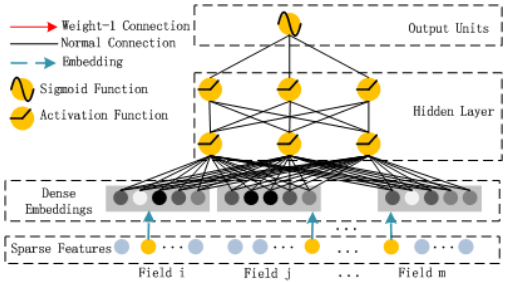
\includegraphics[width=.8\textwidth]{pics/deepfm-deep.png}
	\caption{The architecture of DNN}
	\label{fig:deepfm-deep}
\end{figure}
Deep部分的结构如Fig.\ref{fig:deepfm-deep}所示。由于大部分特征都是稀疏的,为了输入神经网络中,Dense Embedding将稀疏的特征转化成稠密的向量。Dense Embedding的结构如Fig.\ref{fig:deepfm-embedding}所示。

\begin{figure}[h]
	\centering
	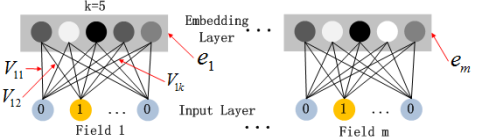
\includegraphics[width=.8\textwidth]{pics/deepfm-embedding.png}
	\caption{The structure of the embedding layer}
	\label{fig:deepfm-embedding}
\end{figure}
Dense Embedding层将$x_{field}$向量编码成低维的稠密向量,其计算过程如Fig.\ref{fig:embedding}所示。$e_{i} = x_i \cdot \boldsymbol{V}$,其中$x_i \in \mathbb{R}^n$是$field i$的向量表示,$\boldsymbol{V} \in \mathbb{R}^{n \times k}$每行表示一个特征的隐向量,$n$表示$field i$的特征数。很显然,\textbf{Dense Embedding层将$\boldsymbol{V}$作为参数}。如果$x_{i}$是one-hot,则$e_i$表示第$i$个特征的隐向量,即\textbf{将不为零的那个特征的隐向量作为其Dense Embedding的输出}。最终Dense Embedding的输出为:$a^{(0)} = [e_1, e_2, ..., e_m]$,$a^{(0)}$作为Hidden Layer的输入,接下来就是常规操作啦。

在Deep部分,可以学习到高阶的交叉特征。

\begin{figure}[h]
	\centering
	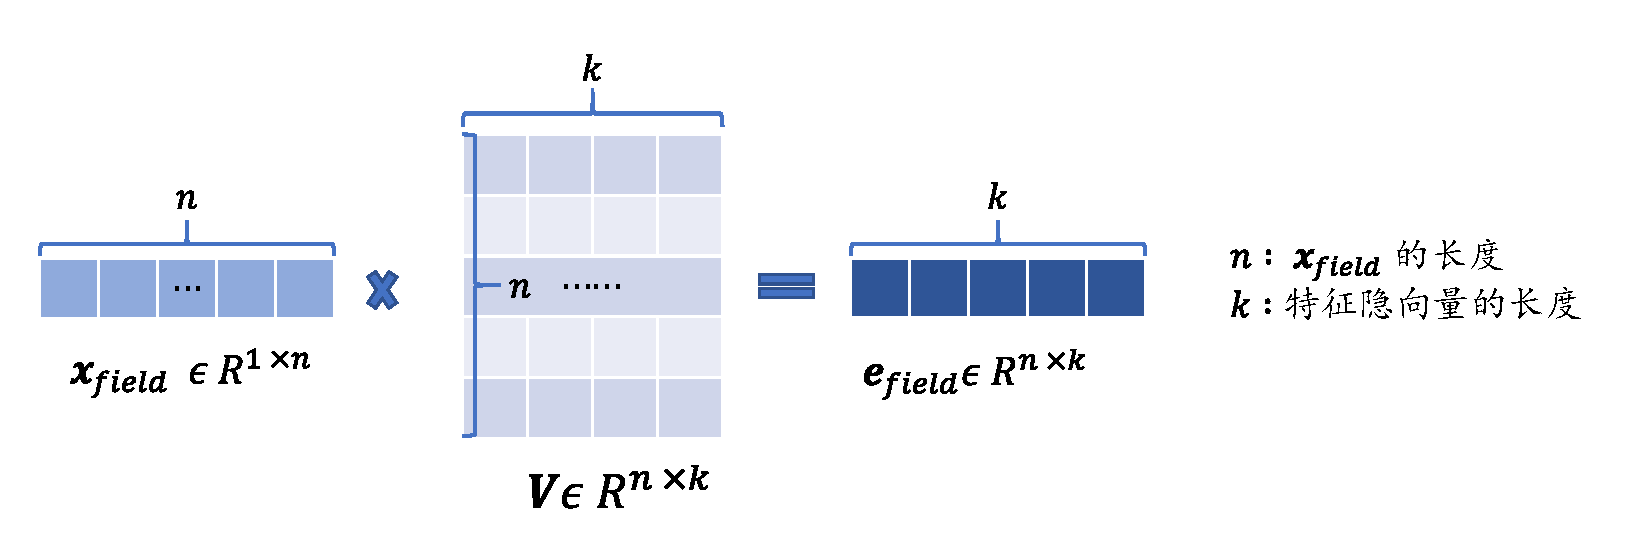
\includegraphics[width=.8\textwidth]{pics/embedding.pdf}
	\caption{Dense Embedding层计算方式}
	\label{fig:embedding}	
\end{figure}


最终,FM部分和Deep部分是联合训练的,整个模型的参数包括$w_i, \boldsymbol{V}, (\boldsymbol{W}^{(l)}, b^{(l)})$。

\paragraph{总结}

\begin{itemize}

	\item 与现有的一些模型,如FNN,不需要预先训练FM部分的隐向量,DeepFM通过联合训练得到隐向量
	\item DeepFM的FM和Deep部分共享输入
		

\end{itemize}

